\documentclass[12pt,a4paper]{article}
\usepackage[utf8]{inputenc}
\usepackage[spanish, es-tabla]{babel}
\usepackage{mathptmx}%fuente Times
\usepackage{sectsty}
\allsectionsfont{\fontfamily{phv}\selectfont}
\chapterfont{\fontfamily{phv}\selectfont}
\usepackage{float}
\usepackage{graphicx}
\graphicspath{ {imagenes/} }
% Metadata para el PDF a generar 
\usepackage[unicode,
pdftex]{hyperref}
\hypersetup{
	pdfauthor={Pablo Sebastián Benítez González},
	pdftitle={Proceso para subir la aplicación en Release},
	pdfsubject={},
	pdflang={es-UY},
	pdfproducer={TeXstudio}
}
\hypersetup{
	colorlinks=true,
	urlcolor=blue,
	linkcolor=black,
	citecolor=black
}
%opening
\title{Proceso para subir la aplicación en Release\\v1.1}
\author{Pablo Sebastián Benítez González}
\date{31 de Octubre\\2020}

\begin{document}

\maketitle

\tableofcontents

\clearpage

\begin{abstract}
Este breve \textbf{documento es una guía} para crear el release de la aplicación para ser entregada. No es un documento exhaustivo sobre el proceso. Intenta ser una referencia rápida para ejecutar el proceso de entrega del \textbf{Obligatorio 1} de \textbf{Diseño de aplicaciones} dictado \textbf{Agosto 2020}.

Este documento no suple los documentos oficiales provistos por la Cátedra. Además del \texttt{Release} en \textit{GitHub} se debe hacer entrega por Gestión.

Este documento refiere únicamente al proceso técnico de crear el \texttt{Release} y el \texttt{tag} en \textit{GitHub}.
\end{abstract}

\section{Chequeo antes de comenzar}

Detalles a verificar \textbf{antes} de armar el release.

\begin{itemize}
	\item Features y otras ramas. \textbf{Todas mergeadas a develop}
	\item Documentación actualizada, verificada y generada en formato \textit{PDF}.
	\begin{itemize}
		\item Revisar los diagramas \textit{UML} y comprobar que estén al día con el código fuente.
		\item Actualizar \textit{Tabla de contenidos}.
		\item Verificar que en el documento está la \textit{URL} al repositorio del grupo dentro de la organización \texttt{ORT-DA1}.
	\end{itemize}
\end{itemize}

\section{Desplegar la aplicación}
\subsection*{Visual Studio}\label{despliegueVS}
\begin{enumerate}
	\item Traer los cambios del remoto.
	\begin{enumerate}
		\item \texttt{git checkout develop}
		\item \texttt{git pull}
	\end{enumerate}
	\item Verificar que todo haya sido exitoso y que no haya conflictos.
	\item Desde el menú, ejecutar \texttt{Build - Clean Solution}
	\begin{figure}[H]		\centering \fbox{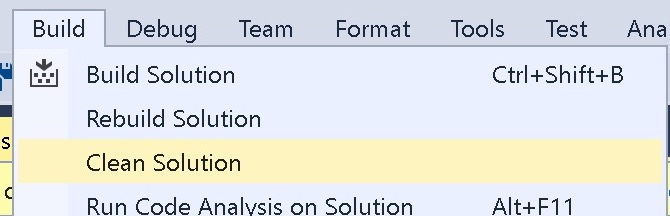
\includegraphics[width=0.5\textwidth]{CleanSolution.jpg}} \end{figure}
	\item Cambiar el modo de compilación a \texttt{Release}.
		\begin{figure}[H]		\centering \fbox{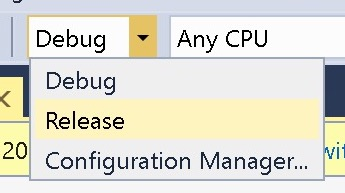
\includegraphics[width=0.4\textwidth]{Release.jpg}} 
		\end{figure}
	\item Desde el menú, ejecutar \texttt{Build - Build Solution} (Ctrl+Shift+B)
	\begin{enumerate}
		\item Verificar que la compilación fué exitosa. Esto se puede hacer revisando la salida de la ventana \texttt{Output} dentro de \textit{Visual Studio}.
	\end{enumerate}
	\item Navegar a la carpeta que contiene el proyecto de \textbf{\textit{Windows Forms}}. En la ventana \texttt{Output} \textit{Visual Studio} nos indica la ruta al archivo \texttt{.exe} generado.
	\begin{enumerate}\label{carpetaRelease}
		\item La carpeta \texttt{bin{\textbackslash}Release} contiene todo lo necesario para ejecutar su aplicación. Toda la carpeta es necesaria.
	\end{enumerate}
	\item Ejecutar el archivo \texttt{.exe}.
	\begin{enumerate}
	\item Corroborar que la aplicación funciona correctamente y que no se cae. Usarla e interactuar con ella.
	\item Es recomendable copiar la carpeta \texttt{Release} a otra computadora y probarla nuevamente para verificar que no hay dependencias con la computadora de desarrollo.
	\end{enumerate}	
	 
\end{enumerate}
\clearpage
\section{Release en GitHub}
\begin{enumerate}
	\item Si estamos siguiendo Gitflow \footnote{\href{https://www.atlassian.com/git/tutorials/comparing-workflows/gitflow-workflow}{Gitflow - Release Branches}} deberíamos crear una rama \texttt{release}.  
	\begin{enumerate}
		\item \texttt{git checkout develop}
		\item \texttt{git pull} (por si acaso)
		\item \texttt{git checkout -b release/entrega\_1}
		\item \texttt{git checkout master}
		\item \texttt{git pull} (por si acaso)
		\item \texttt{git merge release/entrega\_1}
		\item \texttt{git push}
	\end{enumerate}
	
	\item Creamos el \texttt{tag} y el release en GitHub
	\begin{enumerate}
		\item Visitar: \texttt{https://github.com/ORT-DA1/\textit{my-repositorio}/releases/new}
		\begin{enumerate}
			\item En \textbf{Target:} debemos elegir \textbf{master}.
			\item En \textbf{Tag version}, ingresar \textbf{entrega\_1}
			\item En \textbf{Release title}, ingresar un nombre para su entrega.
			\item En \textbf{Write}, ingresar texto libre referente a su entrega.
			\item En \textbf{Attach binaries by dropping them here or selecting them}:
			\begin{enumerate}
				\item Subir un \textit{ZIP} de la carpeta \texttt{Release} (ver \autoref{carpetaRelease})
				\item Subir la documentación digital en formato \textit{PDF}.
			\end{enumerate}		
			\item Click en \textbf{Publish release}.	
		\end{enumerate}
	\end{enumerate}
		\begin{figure}[H]		\centering \fbox{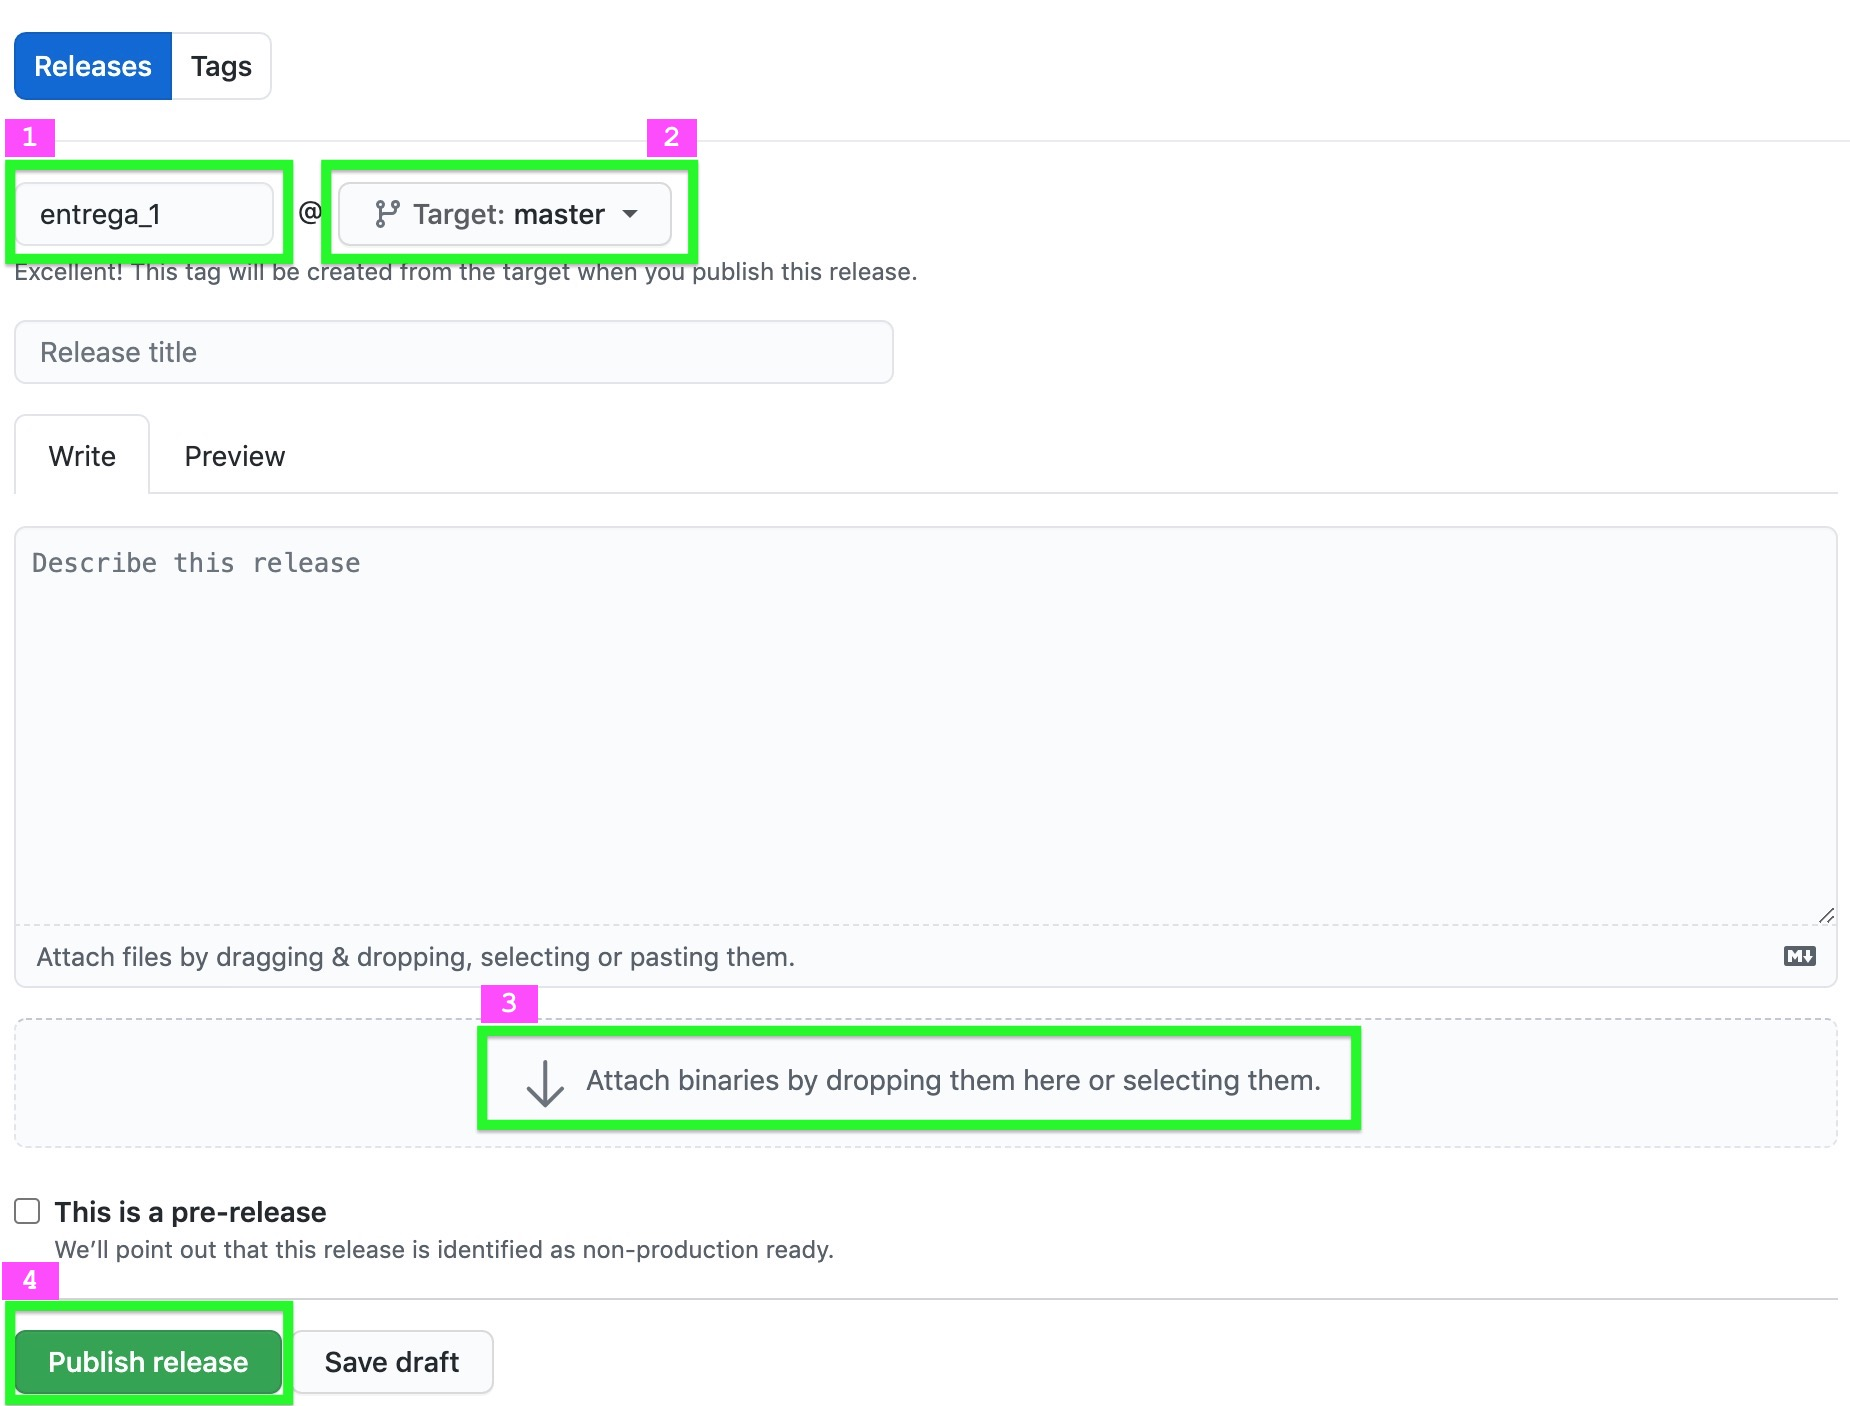
\includegraphics[width=0.8\paperwidth]{GitHub.jpg}} 
\end{figure}
\end{enumerate}

\section{Posibles problemas}

\paragraph{Si nos quedaron ramas sin mergear a develop}
Crear un pull request por cada rama y mergear a \texttt{develop}.

\paragraph{Fallos al comprobar funcionamiento en Release}
Si luego de compilar encontramos fallos en la aplicación y es necesario hacer bug fixing ver la sección \texttt{Hotfix Branches} \footnote{\href{https://www.atlassian.com/git/tutorials/comparing-workflows/gitflow-workflow}{Gitflow - Hotfix Branches}}. En todo caso, de forma mas simple, se podría simplement hacer un branch \texttt{hotfix\_$\cdots$} saliendo desde \texttt{develop}. Luego mergear con un \texttt{Pull Request} en github on manualmente de forma local y volver a \autoref{despliegueVS}.

\end{document}
